\chapter{Documentación adicional}
\section{Fichas de registro} \label{sec:registrationforms}
En este documento, se sitúan todos los campos necesarios para la recogida de datos de campo
y de registro completo. Así, en él se reflejan las \textbf{UE reducidas}, \textbf{UE
estratigráficas de registro completo},  \textbf{hechos}, \textbf{estancias}, el
\textbf{inventario fotográfico}, \textbf{mobiliario}, \textbf{cerámica} y \textbf{tipología},
aunque estos tres últimos no los abarcaremos en este proyecto. \\

Este documento que se adjunta en primer lugar en la página siguiente \textbf{NO es de
autoría propia} y fue un documento proporcionado por el arqueólogo como apoyo documental.

\section{Metodología de registro}
En este documento, la parte principal y más importante describe \textbf{cómo se identifican
las entidades}, indicando el tipo de campos a los que se corresponden: enteros, palabras ya
previamente definidas, como por ejemplo la letra identificativa de los hechos junto con la
numeración, etc. Esta información será de gran utilidad a la hora de elaborar el modelo E/R
y tener claro qué atributos forman la clave primaria y posibles claves candidatas de las
entidades. \\

Este documento se adjunta en segundo lugar, después de \ref{sec:registrationforms}, e
igual que el anterior, \textbf{NO es de autoría propia} y fue un documento proporcionado por
el arqueólogo como apoyo documental.

% Fichas de recogida de datos, tanto de campo como completas
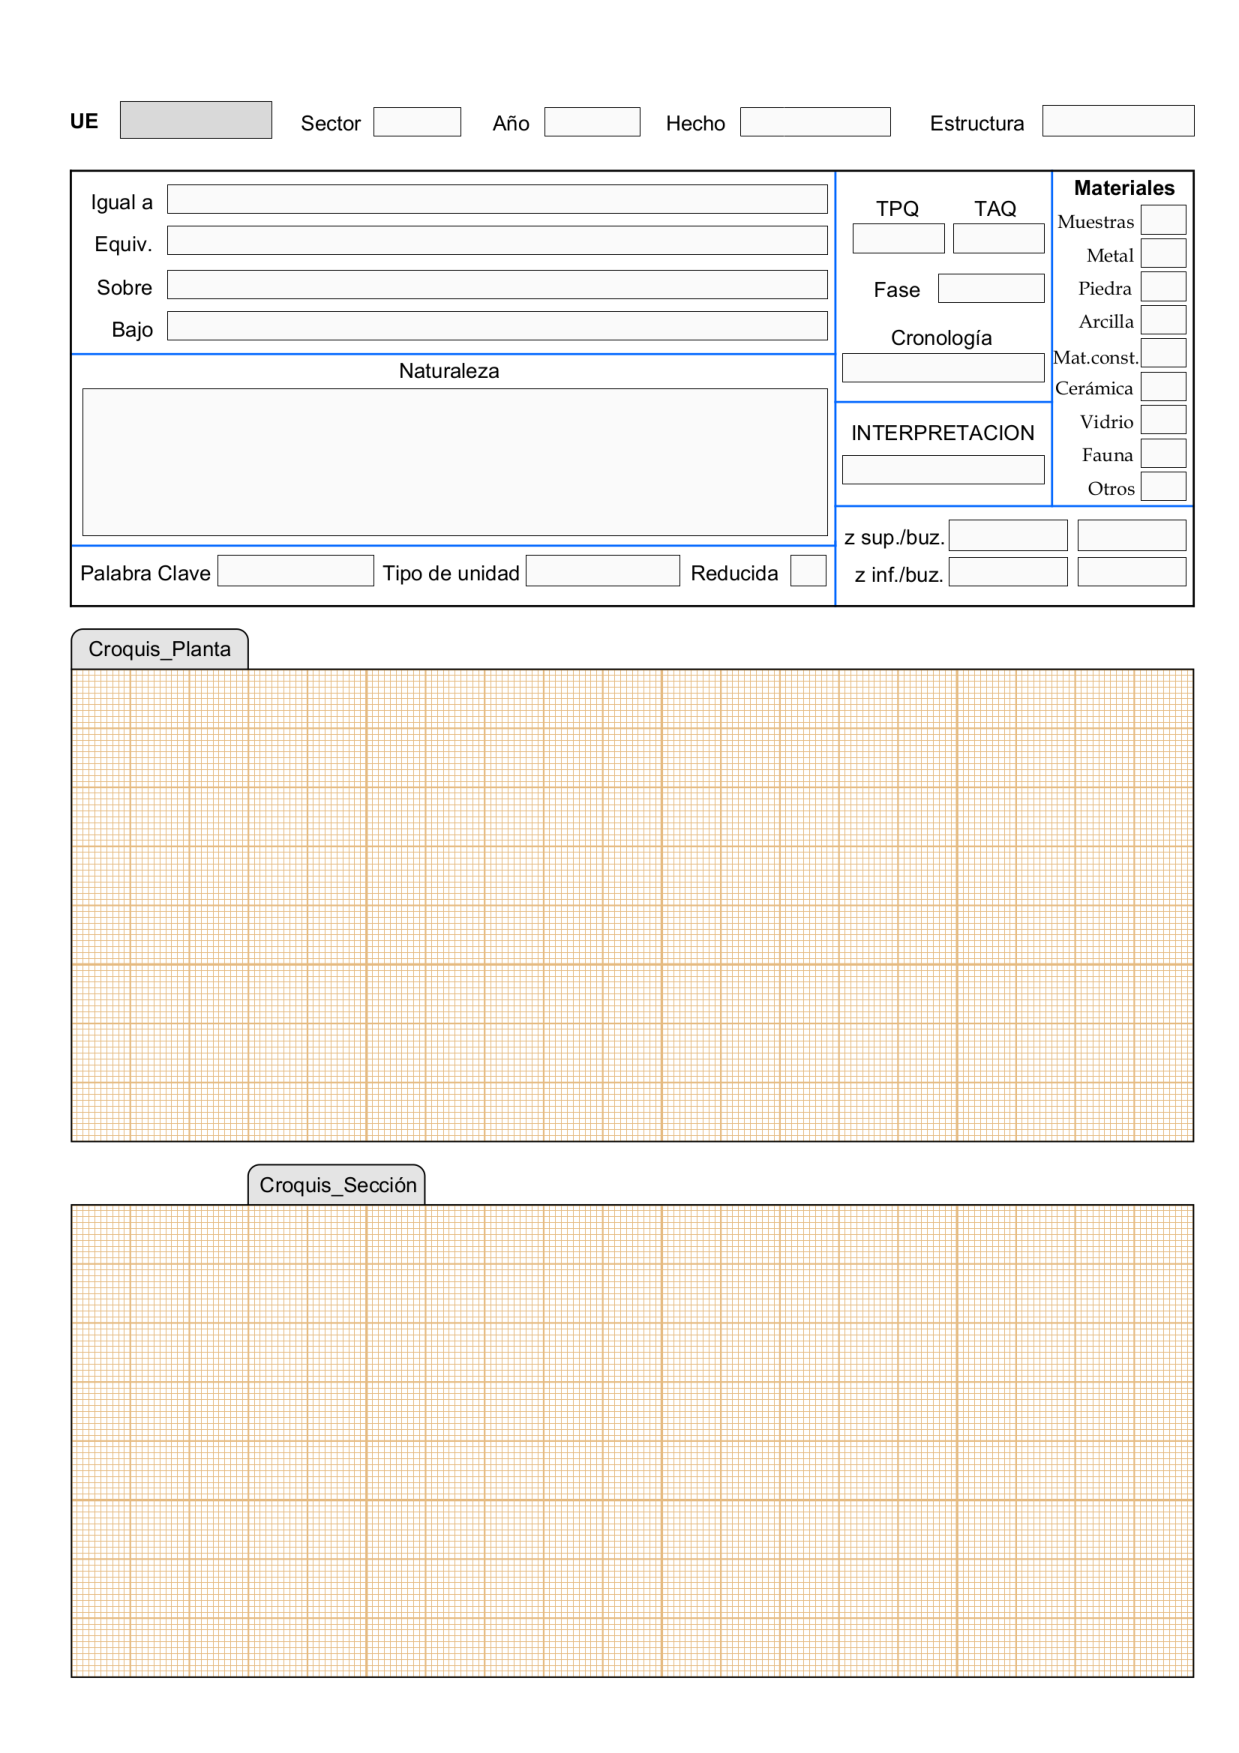
\includepdf[pages=-]{info/FichasRegistroCampoCompleto.pdf}

% Jerarquía entre los elementos e identificación de ellos
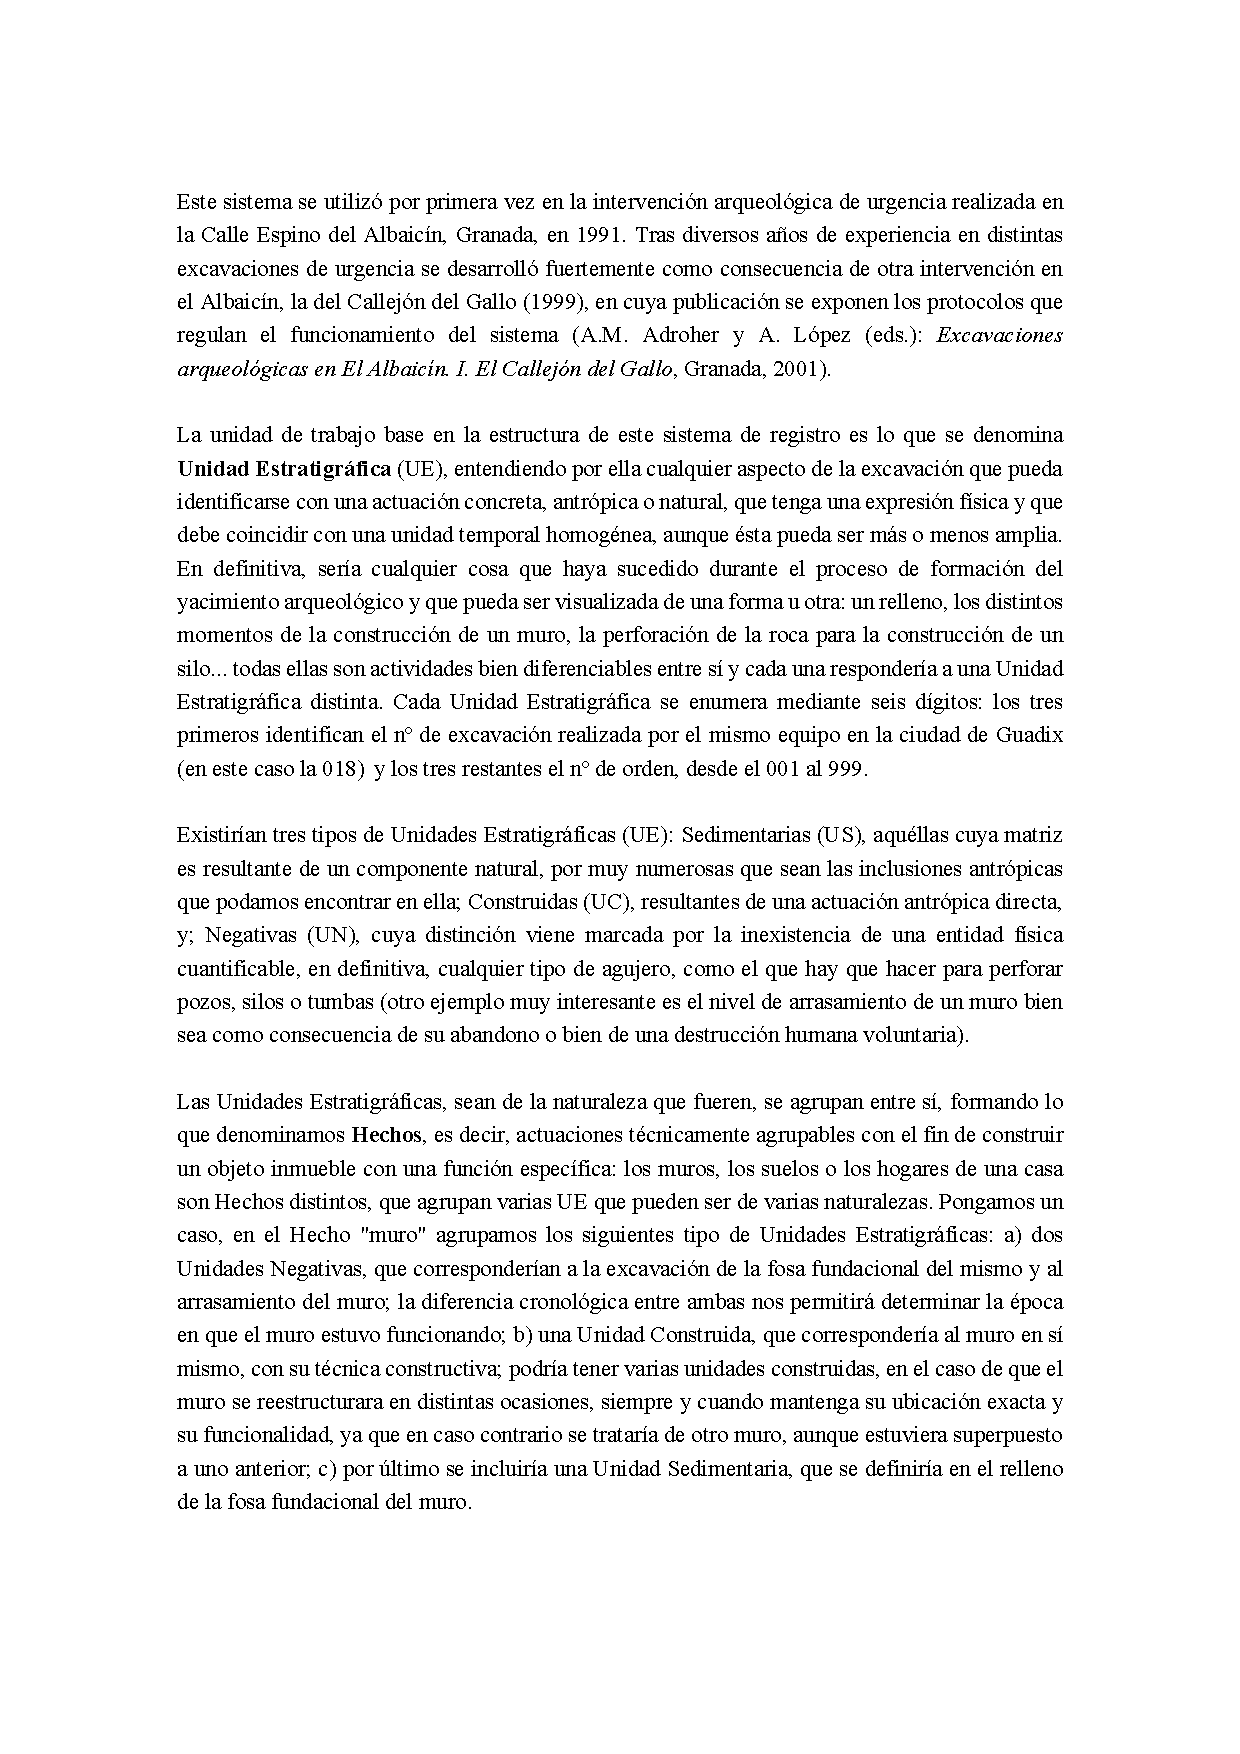
\includepdf[pages=-]{info/MetodologiaFichasRegistro.pdf}
